\subsection{Ondas estacionárias de som: geração de harmônicos
em função da frequência f}

Conforme descrito na Metodologia, neste experimento o gerador de ondas com o pistão e o microfone foi ligado com um L fixo aproximadamente igual a: L = ($0,110 \pm 0,001$) m. Os harmônicos são gerados no tubo, do harmônico fundamental (n = 1) até n = 5. Foram observadas mudanças nas ondas, devido a mudança de pressão.  Para o início do experimento, as frequências variaram do menor valor ao maior valor possível, para a detecção dos harmônicos fundamentais, e foram registradas na Tabela a seguir:

\begin{table}[H]
    \centering
    \begin{tabular}{ |c||c||c|  }
        \hline
        \textbf{Índice do harmônico \textit{n}} & \textbf{Frequência \textit{$f_n$}(kHz)} & \textbf{$n/2L$}\\
        \hline 
         1&	1,5634&	4,5454	\\
         
         2&	3,0625&	9,0909 \\
         
         3&	4,5149&	13,6364 \\
         
         4&	6,0410&	18,1818 \\
         
         5&	7,5049&	22,7273 \\
        \hline
    \end{tabular}
    \caption{Valores registrados para as frequências $f_n$ correspondente aos sucessivos harmônicos n.} 
\end{table}

Após o registro dos dados acima, construímos o gráfico relacionando as frequências $f_n$ em função de $n/2L$, que pode ser observado abaixo:

\begin{figure}[H]
  \centering
  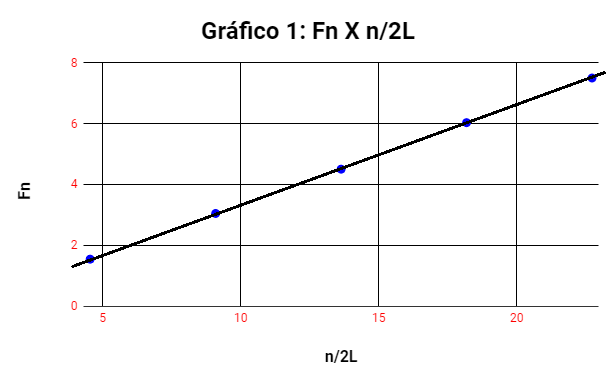
\includegraphics[scale=0.8]{images/gráfico 1.png}
  \caption{ Gráfico de $f_n$ em função de $n/2L$.}
\end{figure}

Com base no gráfico, é possível observar que há uma relação de linearidade entre os pontos, podendo uni-los sob uma única reta. Portanto, podemos concluir que o gráfico obtido é coerente com as equações que definem a onda estacionária visto que todas são de primeiro grau (ou seja, formam uma reta) e obtidas da relação entre o frequência de onda, velocidade e o harmônico correspondente: $f_n=v \cdot n/2L$.

Analisando os dados obtidos no gráfico, podemos aplicar o método dos mínimos quadrados para determinar a velocidade do som no ar, já que na equação da onda estacionária a velocidade corresponde ao coeficiente angular. Para isso, utilizaremos um aplicativo (Least Squares) desenvolvido por nosso colega de turma André Zanardi Creppe que calcula os valores dos coeficientes de reta a partir dos mínimos quadrados. Segue abaixo uma captura de tela do resultado obtido após a inclusão dos nossos dados no aplicativo:

\begin{figure}[H]
  \centering
  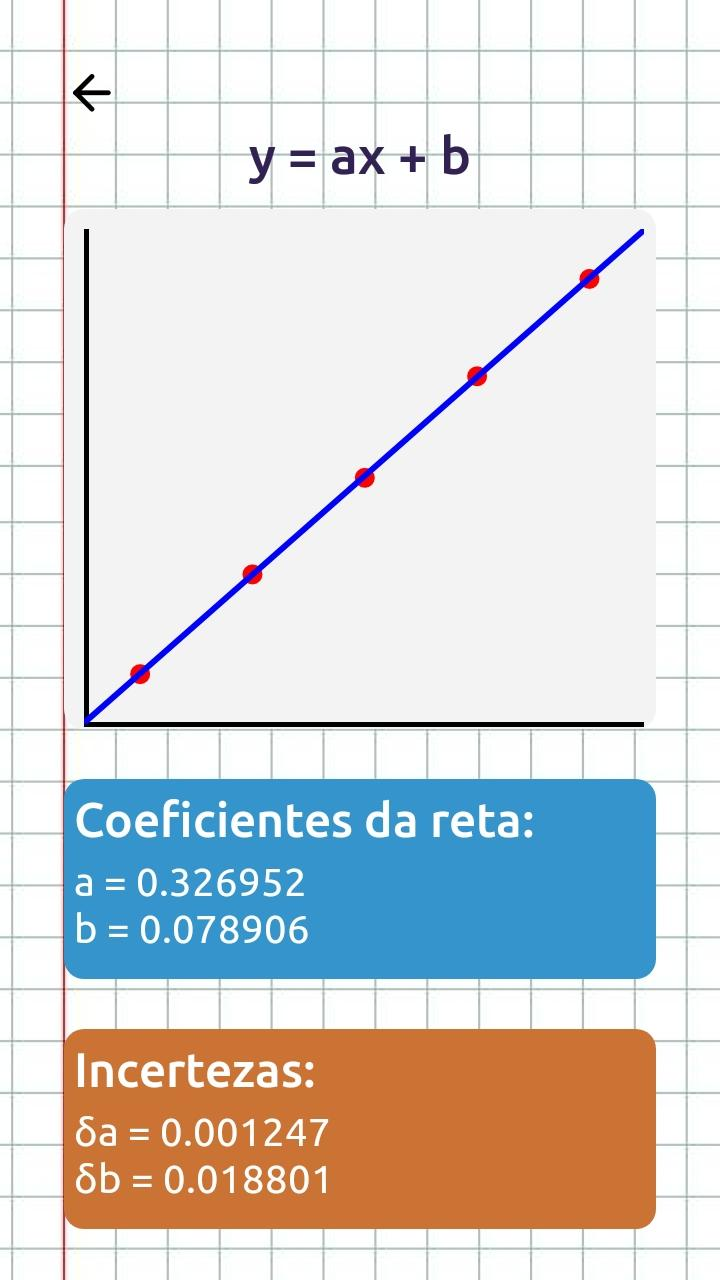
\includegraphics[scale=0.25]{images/Gráfico 2.jpeg}
  \caption{ Aplicação dos Mínimos Quadrados para obtenção dos coeficientes da reta.}
\end{figure}

Após a análise gráfica da relação entre a frequência e o harmônico da onda, aplicando o método dos mínimos quadrados, o coeficiente angular assumiu o valor de a =$(0,327 \pm 0,001)\cdot 10^3$ . Já o coeficiente linear foi igual a: $b =(0,08 \pm 0,01)\cdot 10^3$.

Dessa forma, como o coeficiente angular corresponde à velocidade na equação de onda estacionária, temos que a velocidade do som no ar, obtido no experimento para uma temperatura local de 25ºC, foi igual a:

\[ \therefore v = (0,327 \pm 0,001) \cdot 10^3 = (327 \pm 1) m/s^2 \] 

Sabendo que o valor de referência da velocidade do som no ar para temperatura de 25ºC é aproximadamente igual a $v_{ref}= 343 m/s$, temos que a velocidade encontrada no experimento não corresponde com o valor tabelado na literatura. Entretanto, podemos observar que o valor obtido é próximo ao valor real, registrando uma pequena diferença. Essa diferença pode ser justificada por meio de erros sistemáticos cometidos ao longo da experiência ou por sucessivas aproximações que levaram a uma dispersão dos valores.

Dessa forma, conclui-se que o experimento não ofereceu condições ou dados suficientes para a obtenção de um valor real ou próximo da referência. Para que isso acontecesse, podemos assumir que o coeficiente linear deveria assumir um valor igual a zero já que na equação de ondas estacionárias ($f_n = v \cdot \frac{n}{2L}$) não há coeficiente linear. Esse levantamento não é coerente com o resultado do nosso experimento, pois obtemos um valor diferente de zero para o coeficiente linear após a aplicação dos mínimos quadrados.

Para garantir que o primeiro harmônico observado corresponde ao harmônico fundamental n=1, podemos realizar o processo inverso partindo da velocidade de onda do som no ar para obter a frequência. Para isso, sabemos os valores da velocidade ($v_{ref} = 343 m/s^2$), do comprimento da coluna de ar (L = 0,11 m) e o harmônico (n=1). Então, temos:

\[  f'_1 = v \cdot \frac{n}{2L} = 343 \cdot \frac{1}{2 \cdot 0,11} \]
\[  f'_1 = 343 \cdot \frac{1}{0,22} = 343 \cdot 4,5454 \]
\[  \therefore f'_1 = 1559,09 Hz = (1,5591) kHz \]

Com base nos cálculos realizados e sabendo que a frequência do harmônico fundamental registrado experimentalmente é igual a $f_1 = 1,5634$, podemos concluir que a frequência esperada $f'_1$ não coincide com o menor valor de frequência tabelado. Isso pode ser explicado por um erro sistemático de leitura do osciloscópio que fornece a imagem das ondas. Um pequeno desvio de interpretação de quando a onda atingiu sua máxima pressão é o suficiente para gerar uma diferença nos valores das frequências do harmônico fundamental.
